\chapter{Oscillator phase noise}
\label{app:OscillatorPhaseNoise}
A precision oscillator is well-described in the complex plane via
\begin{equation}
  A(t)
  =
  \left[ A_0 + \varepsilon(t) \right]
  e^{i \left[ \omega_0 t + \phi(t) \right]},
\end{equation}
where
$A_0$ is the nominal amplitude,
$\varepsilon(t)$ is the deviation from the nominal amplitude,
$\omega_0$ is the nominal angular frequency, and
$\phi(t)$ is the phase deviation from the nominal phase $\omega_0 t$
\cite{ieee_std1139}.
Within the context of this work,
it is sufficient to regard $\varepsilon(t)$ and $\phi(t)$
as zero-mean, stationary, random processes.
Note that both $\varepsilon(t)$ and $\phi(t)$
have simple geometric interpretations,
as shown in Figure~\ref{fig:OscillatorPhaseNoise:oscillator_complex_plane}.
Typically, $|\varepsilon(t)| \ll A_0$ such that
the amplitude deviation can be neglected.
However, phase-sensitive instruments,
such as interferometers,
can be susceptible to small phase deviations.
This appendix discusses
the IEEE definition of phase noise $\mathcal{L}(f)$ and
quantitatively links it
to the corresponding noise of a phase-sensitive instrument.

\begin{figure}[h]
  \centering
  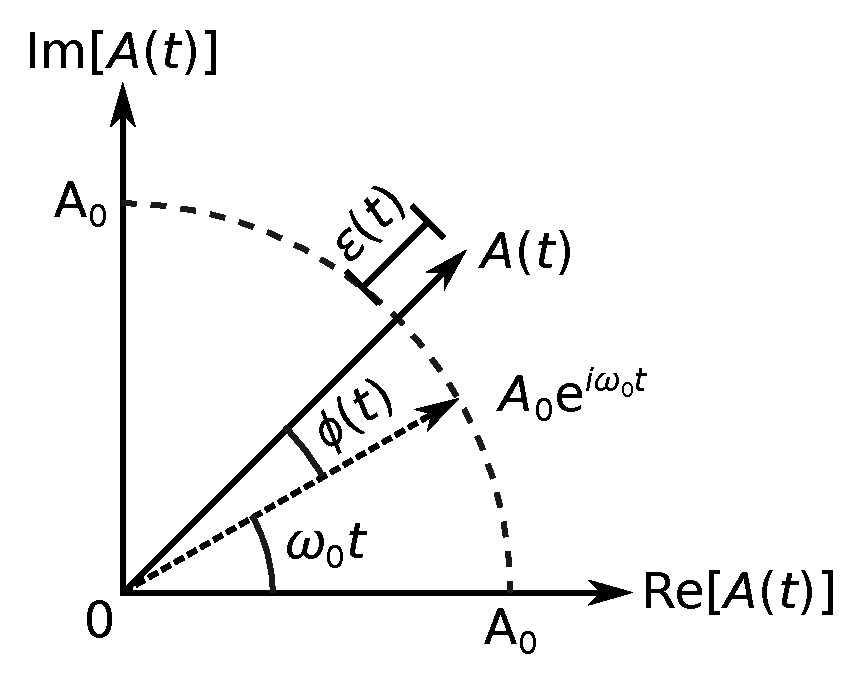
\includegraphics[width = 0.55\textwidth]{%
    Appendices/OscillatorPhaseNoise/figs/oscillator_complex_domain.pdf}
  \caption[Oscillator amplitude and phase deviations in the complex plane]{%
    An oscillator's amplitude deviation $\varepsilon(t)$ and
    phase deviation $\phi(t)$ can be easily visualized in the complex plane.}
\label{fig:OscillatorPhaseNoise:oscillator_complex_plane}
\end{figure}


\section{Definitions}
An oscillator's phase noise $\mathcal{L}(f)$
(pronounced as ``script-ell of $f$'')
is defined as
\begin{equation}
  \mathcal{L}(f)
  =
  \frac{G_{\phi,\phi}(f)}{2},
  \label{eq:OscillatorPhaseNoise:oscillator_phase_noise}
\end{equation}
where $G_{\phi,\phi}(f)$ is
the one-sided autospectral density of the phase fluctuations $\phi(t)$
\cite{ieee_std1139}.
Note that the one-sided autospectral density $G_{\phi,\phi}(f)$
is related to the two-sided autospectral density $S_{\phi,\phi}(f)$ via
\begin{equation}
  G_{\phi, \phi}(f)
  =
  \begin{cases}
    2 S_{\phi, \phi}(f), \quad f > 0
    \\
    S_{\phi, \phi}(f), \quad f = 0
  \end{cases}.
\end{equation}
The two-sided autospectral density $S_{\phi,\phi}(f)$ is itself defined as
\begin{equation}
  S_{\phi,\phi}(f)
  =
  \mathcal{F}\left[ R_{\phi,\phi}(\tau) \right](f),
\end{equation}
where $\mathcal{F}$ is the Fourier transform operator and
$R_{\phi,\phi}(\tau)$ is the autocorrelation function defined as
\begin{equation}
  R_{\phi,\phi}(\tau)
  =
  E\left[ \phi(t) \cdot \phi(t + \tau) \right];
\end{equation}
here, $E$ is the expectation-value operator
\cite[Ch.~5]{bendat_and_piersol}.


\section{Units}
Phase noise $\mathcal{L}(f)$ can be expressed in SI units
as $\SI{}{\radian\squared\per\hertz}$.
However, this is \emph{not} common practice.
Instead, it is much more common to express phase noise in units of
$\SI{}{\decibel c \per\hertz}$, which
corresponds to the ratio (expressed in $\SI{}{\decibel}$)
of phase-noise power to carrier-signal power
in a one $\SI{}{\hertz}$ bandwidth.
Explicitly,
\begin{equation}
  \mathcal{L}(f) \, [\SI{}{\decibel c \per\hertz}]
  =
  10 \log_{10} \left(%
    \mathcal{L}(f) \, [\SI{}{\radian\squared\per\hertz}]
  \right).
\end{equation}
While it may initially come as a surprise that
phase noise should be expressible in terms
of the power in the carrier signal
(i.e.\ the nominal oscillator signal),
this choice of units is perfectly natural.
To see this, examine
Figure~\ref{fig:OscillatorPhaseNoise:oscillator_complex_plane}:
the oscillator's nominal phasor $A_0 e^{i \omega_0 t}$
is displaced in the perpendicular direction
by $A(t) \sin\phi(t) \approx A_0 \phi(t)$, where
the approximation follows for the small amplitude and phase deviations
($|\varepsilon(t)| \ll A_0$, $|\phi(t)| \ll 1$) of practical relevance.
Thus, a phase deviation $\phi(t)$ produces a phasor deviation
that is proportional to the oscillator's nominal amplitude $A_0$,
making $\SI{}{\decibel c \per\hertz}$
a natural choice of units for $\mathcal{L}(f)$.


\section{Connection to instrumental phase noise}
Numerous phase-sensitive instruments,
such as interferometers, demodulators, etc.\,
operate by comparing an oscillator's phase
at times $t$ and $t + \tau_j$:
\begin{equation}
  \arg[A^*(t) \cdot A(t + \tau_j)]
  =
  \omega \tau_j + \delta \phi(t, \tau_j),
\end{equation}
where $\omega \tau_j$ is the expected phase progression and
\begin{equation}
  \delta \phi(t, \tau_j) = \phi(t + \tau_j) - \phi(t)
\end{equation}
is the \emph{instrumental} phase noise.
Obviously, the instrumental phase noise $\delta\phi(t, \tau_j)$
is very closely related to the oscillator phase deviation $\phi(t)$, and
it is the goal of this section
to quantitatively relate the autospectral density
of the instrumental phase noise $S_{\delta\phi,\delta\phi}(f)$
to the oscillator phase noise $\mathcal{L}(f)$.


\subsection{Autocorrelation of instrumental phase noise}
The autocorrelation of the instrumental phase noise
$R_{\delta\phi,\delta\phi}(\tau)$ is
\begin{align}
  R_{\delta\phi,\delta\phi}(\tau)
  &=
  E\left[
    \delta\phi(t, \tau_j)
    \cdot
    \delta\phi(t + \tau, \tau_j)
  \right]
  \notag \\
  &=
  E\left[%
    \left\{ \phi(t + \tau_j) - \phi(t) \right\}
    \cdot
    \left\{ \phi(t + \tau + \tau_j) - \phi(t + \tau) \right\}
  \right]
  \notag \\
  &=
  E\left[%
    \phi(t + \tau_j) \cdot \phi(t + \tau + \tau_j)
  \right]
  -
  E\left[%
    \phi(t + \tau_j) \cdot \phi(t + \tau)
  \right]
  \notag \\
  &\quad-
  E\left[%
    \phi(t) \cdot \phi(t + \tau + \tau_j)
  \right]
  +
  E\left[%
    \phi(t) \cdot \phi(t + \tau)
  \right]
  \notag \\
  &=
  2 R_{\phi,\phi}(\tau)
  -
  R_{\phi,\phi}(\tau + \tau_j)
  -
  R_{\phi,\phi}(\tau - \tau_j),
  \label{eq:OscillatorPhaseNoise:instrumental_phase_noise_autocorrelation}
\end{align}
where (\ref{eq:OscillatorPhaseNoise:instrumental_phase_noise_autocorrelation})
follows from the stationary nature of the phase deviation $\phi(t)$ and
the invariance of a stationary process's autocorrelation function
to translations in time.


\subsection{Autospectral density of instrumental phase noise}
The autospectral density of the instrumental phase noise
$S_{\delta\phi,\delta\phi}(f)$
is simply the Fourier transform
of the corresponding autocorrelation function
(\ref{eq:OscillatorPhaseNoise:instrumental_phase_noise_autocorrelation}).
Explicitly,
\begin{align}
  S_{\delta\phi,\delta\phi}(f)
  &=
  \mathcal{F}\left[ R_{\delta\phi,\delta\phi}(\tau) \right](f)
  \notag \\
  &=
  2 \mathcal{F}\left[ R_{\phi,\phi}(\tau) \right](f)
  -
  \mathcal{F}\left[ R_{\phi,\phi}(\tau + \tau_j) \right](f)
  \notag \\
  &\quad-
  \mathcal{F}\left[ R_{\phi,\phi}(\tau - \tau_j) \right](f)
  \notag \\
  &=
  2 S_{\phi,\phi}(f)
  -
  \left( e^{i 2 \pi f \tau} + e^{-i 2 \pi f \tau} \right) S_{\phi,\phi}(f)
  \notag \\
  &=
  2 \left[ 1 - \cos(2 \pi f \tau_j) \right] S_{\phi,\phi}(f)
  \notag \\
  &=
  4 \sin^2(\pi f \tau_j) S_{\phi,\phi}(f),
  \label{eq:OscillatorPhaseNoise:instrumental_phase_noise_2sided_autospectral_density}
\end{align}
where the Fourier transform's linear and
translational properties have been used.
Referencing the definition of oscillator phase noise
(\ref{eq:OscillatorPhaseNoise:oscillator_phase_noise}),
the instrumental phase noise
(\ref{eq:OscillatorPhaseNoise:instrumental_phase_noise_2sided_autospectral_density})
can be rewritten (as a one-sided autospectral density) as
\begin{equation}
  G_{\delta\phi,\delta\phi}(f)
  =
  8 \sin^2(\pi f \tau_j) \mathcal{L}(f).
  \label{eq:OscillatorPhaseNoise:instrumental_phase_noise_1sided_autospectral_density}
\end{equation}


\bibliographystyle{plainurl}
\bibliography{references}
